\documentclass[../main.tex]{subfiles}
\begin{document}
	\chapter{Implementation}
	\label{chap:chap_4}
	\noindent Based on the experience from the previous example, it makes sense to write
	some code to automate the analytical integration process for any choice of finite
	element basis functions. In addition, we can automate the assembly process
	and linear system solution. Appropriate functions for this purpose document
	all details of all steps in the finite element computations and can found in the
	module file \href{https://github.com/hplgit/INF5620/blob/master/src/fem/fe_approx1D.py}{fe\textunderscore approx1D.py.} The key steps in the computational machinery are
	now explained in detail in terms of code and text.
	\section[Integration]{Integration}
	\label{sec:sec_4_1}
	First we need a Python function for defining $\tilde{\varphi}_{r}(X)$ in terms of a Lagrange polynomial of degree $d$ :
	\begin{lstlisting}[numbers=none]
		import sympy as sp
		import numpy as np
		def phi_r(r, X, d):
		if isinstance(X, sp.Symbol):
		h = sp.Rational(1, d) # node spacing
		nodes = [2*i*h - 1 for i in range(d+1)]
		else:
		# assume X is numeric: use floats for nodes
		nodes = np.linspace(-1, 1, d+1)
		return Lagrange_polynomial(X, r, nodes)
		
		def Lagrange_polynomial(x, i, points):
		p = 1
		for k in range(len(points)):
		if k != i:
		p *= (x - points[k])/(points[i] - points[k])
		return p	
	\end{lstlisting}
	Observe how we construct the phi\textunderscore r function to be a symbolic expression for $\tilde{\varphi}_{r}(X)$ if $\mathrm{X}$ is a Symbol object from sympy. Otherwise, we assume that $\mathrm{X}$ is a float object and compute the corresponding floating-point value of $\ddot{\varphi}_{r}(X)$. Recall that the Lagrange\textunderscore polynomial function, here simply copied from Section \hyperref[sec:sec_2_7]{2.7}, works with both symbolic and numeric variables.
	
	The complete basis $\tilde{\varphi}_{0}(X), \ldots, \tilde{\varphi}_{d}(X)$ on the reference element, represented as a list of symbolic expressions, is constructed by
	\begin{lstlisting}[numbers=none]
		def basis(d=1):
		X = sp.Symbol('X')
		phi = [phi_r(r, X, d) for r in range(d+1)]
		return phi	
	\end{lstlisting}
	Now we are in a position to write the function for computing the element matrix:
	\begin{lstlisting}[numbers=none]
		def element_matrix(phi, Omega_e, symbolic=True):
		n = len(phi)
		A_e = sp.zeros((n, n))
		X = sp.Symbol('X')
		if symbolic:
		h = sp.Symbol('h')
		else:
		h = Omega_e[1] - Omega_e[0]
		detJ = h/2 # dx/dX
		for r in range(n):
		for s in range(r, n):
		A_e[r,s] = sp.integrate(phi[r]*phi[s]*detJ, (X, -1, 1))
		A_e[s,r] = A_e[r,s]
		return A_e	
	\end{lstlisting}
	In the symbolic case (symbolic is True), we introduce the element length as
	a symbol h in the computations. Otherwise, the real numerical value of the element interval Omega\textunderscore e is used and the final matrix elements are numbers, not
	symbols. This functionality can be demonstrated:
	\begin{lstlisting}[numbers=none]
		>>> from fe_approx1D import *
		>>> phi = basis(d=1)
		>>> phi
		[1/2 - X/2, 1/2 + X/2]
		>>> element_matrix(phi, Omega_e=[0.1, 0.2], symbolic=True)
		[h/3, h/6]
		[h/6, h/3]
		>>> element_matrix(phi, Omega_e=[0.1, 0.2], symbolic=False)
		[0.0333333333333333, 0.0166666666666667]
		[0.0166666666666667, 0.0333333333333333]	
	\end{lstlisting}
	The computation of the element vector is done by a similar procedure:
	\begin{lstlisting}[numbers=none]
		def element_vector(f, phi, Omega_e, symbolic=True):
		n = len(phi)
		b_e = sp.zeros((n, 1))
		# Make f a function of X
		X = sp.Symbol('X')
		if symbolic:
		h = sp.Symbol('h')
		else:
		h = Omega_e[1] - Omega_e[0]
		x = (Omega_e[0] + Omega_e[1])/2 + h/2*X # mapping
		f = f.subs('x', x) # substitute mapping formula for x
		detJ = h/2 # dx/dX
		for r in range(n):
		b_e[r] = sp.integrate(f*phi[r]*detJ, (X, -1, 1))
		return b_e	
	\end{lstlisting}
	Here we need to replace the symbol $x$ in the expression for $f$ by the mapping formula such that $f$ can be integrated in terms of $X$, cf. the formula $\tilde{b}_{r}^{(e)}=$ $\int_{-1}^{1} f(x(X)) \tilde{\varphi}_{r}(X) \frac{h}{2} d X$.
	
	The integration in the element matrix function involves only products of polynomials, which sympy can easily deal with, but for the right-hand side sympy may face difficulties with certain types of expressions $f$. The result of the integral is then an Integral object and not a number or expression as when symbolic integration is successful. It may therefore be wise to introduce a fallback on numerical integration. The symbolic integration can also take much time before an unsuccessful conclusion so we may also introduce a parameter symbolic and set it to False to avoid symbolic integration:
	\begin{lstlisting}[numbers=none]
		def element_vector(f, phi, Omega_e, symbolic=True):
		...
		if symbolic:
		I = sp.integrate(f*phi[r]*detJ, (X, -1, 1))
		if not symbolic or isinstance(I, sp.Integral):
		h = Omega_e[1] - Omega_e[0] # Ensure h is numerical
		detJ = h/2
		integrand = sp.lambdify([X], f*phi[r]*detJ)
		I = sp.mpmath.quad(integrand, [-1, 1])
		b_e[r] = I
		...
	\end{lstlisting}
	Numerical integration requires that the symbolic integrand is converted to a plain
	Python function (integrand) and that the element length h is a real number.
	\section[Linear system assembly and solution]{Linear system assembly and solution}
	\label{sec:sec_4_2}
	The complete algorithm for computing and assembling the elementwise contributions takes the following form
	\begin{lstlisting}[numbers=none]
		def assemble(nodes, elements, phi, f, symbolic=True):
		N_n, N_e = len(nodes), len(elements)
		if symbolic:
		A = sp.zeros((N_n, N_n))
		b = sp.zeros((N_n, 1)) # note: (N_n, 1) matrix
		else:
		A = np.zeros((N_n, N_n))
		b = np.zeros(N_n)
		for e in range(N_e):
		Omega_e = [nodes[elements[e][0]], nodes[elements[e][-1]]]
		
		A_e = element_matrix(phi, Omega_e, symbolic)
		b_e = element_vector(f, phi, Omega_e, symbolic)
		
		for r in range(len(elements[e])):
		for s in range(len(elements[e])):
		A[elements[e][r],elements[e][s]] += A_e[r,s]
		b[elements[e][r]] += b_e[r]
		return A, b	
	\end{lstlisting}
	The nodes and elements variables represent the finite element mesh as explained earlier.
	
	Given the coefficient matrix $\mathrm{A}$ and the right-hand side $\mathrm{b}$, we can compute the coefficients $\left\{c_{i}\right\}_{i \in \mathcal{I}_{s}}$ in the expansion $u(x)=\sum_{j} c_{j} \varphi_{j}$ as the solution vector $c$ of the linear system:
	\begin{lstlisting}[numbers=none]
		if symbolic:
		c = A.LUsolve(b)
		else:
		c = np.linalg.solve(A, b)
	\end{lstlisting}
	When A and b are sympy arrays, the solution procedure implied by A.LUsolve is
	symbolic. Otherwise, A and b are numpy arrays and a standard numerical solver
	is called. The symbolic version is suited for small problems only (small N values)
	since the calculation time becomes prohibitively large otherwise. Normally, the
	symbolic integration will be more time consuming in small problems than the
	symbolic solution of the linear system.
	\section[Example on computing symbolic approximations]{Example on computing symbolic approximations}
	\label{sec:sec_4_3}
	We can exemplify the use of assemble on the computational case from Section \hyperref[sec:sec_3_6]{3.6} with two P1 clcments (lincar basis functions) on the domain $\Omega=[0,1]$. Let us first work with a symbolic element length:
	\begin{lstlisting}[numbers=none]
		>>> h, x = sp.symbols('h x')
		>>> nodes = [0, h, 2*h]
		>>> elements = [[0, 1], [1, 2]]
		>>> phi = basis(d=1)
		>>> f = x*(1-x)
		>>> A, b = assemble(nodes, elements, phi, f, symbolic=True)
		>>> A
		[h/3, h/6, 0]
		[h/6, 2*h/3, h/6]
		[ 0, h/6, h/3]
		>>> b
		[ h**2/6 - h**3/12]
		[ h**2 - 7*h**3/6]
		[5*h**2/6 - 17*h**3/12]
		>>> c = A.LUsolve(b)
		>>> c
		[ h**2/6]
		[12*(7*h**2/12 - 35*h**3/72)/(7*h)]
		[ 7*(4*h**2/7 - 23*h**3/21)/(2*h)]	
	\end{lstlisting}
	\section[Comparison with finite elements and interpolation/- collocation]{Comparison with finite elements and interpolation/- collocation}
	\label{sec:sec_4_4}
	We may, for comparison, compute the c vector corresponding to an interpolation/collocation method with finite element basis functions. Choosing the nodes as points, the principle is
	$$
	u\left(x_{i}\right)=\sum_{j \in \mathcal{I}_{s}} c_{j} \varphi_{j}\left(x_{i}\right)=f\left(x_{i}\right), \quad i \in \mathcal{I}_{s}.
	$$
	The coefficient matrix $A_{i, j}=\varphi_{j}\left(x_{i}\right)$ becomes the identity matrix because basis function number $j$ vanishes at all nodes, except node $j: \varphi_{j}\left(x_{i}=\delta_{i j}\right.$. Therefore, $c_{i}=f\left(x_{i}\right.$.
	
	The associated sympy calculations are
	\begin{lstlisting}[numbers=none]
		>>> fn = sp.lambdify([x], f)
		>>> c = [fn(xc) for xc in nodes]
		>>> c
		[0, h*(1 - h), 2*h*(1 - 2*h)]
	\end{lstlisting}
	These expressions are much simpler than those based on least squares or projection in combination with finite element basis functions.
	\section[Example on computing numerical approximations]{Example on computing numerical approximations}
	\label{sec:sec_4_5}
	The numerical computations corresponding to the symbolic ones in Section \hyperref[sec:sec_4_3]{4.3},
	and still done by sympy and the assemble function, go as follows:
	\begin{lstlisting}[numbers=none]
		>>> nodes = [0, 0.5, 1]
		>>> elements = [[0, 1], [1, 2]]
		>>> phi = basis(d=1)
		>>> x = sp.Symbol('x')
		>>> f = x*(1-x)
		>>> A, b = assemble(nodes, elements, phi, f, symbolic=False)
		>>> A
		[ 0.166666666666667, 0.0833333333333333, 0]
		[0.0833333333333333, 0.333333333333333, 0.0833333333333333]
		[ 0, 0.0833333333333333, 0.166666666666667]
		>>> b
		[ 0.03125]
		[0.104166666666667]
		[ 0.03125]
		>>> c = A.LUsolve(b)
		>>> c
		[0.0416666666666666]
		[ 0.291666666666667]
		[0.0416666666666666]	
	\end{lstlisting}
	The fe\textunderscore approx1D module contains functions for generating the nodes and
	elements lists for equal-sized elements with any number of nodes per element.
	The coordinates in nodes can be expressed either through the element length
	symbol h (symbolic=True) or by real numbers (symbolic=False):
	\begin{lstlisting}[numbers=none]
		nodes, elements = mesh_uniform(N_e=10, d=3, Omega=[0,1],
		symbolic=True)	
	\end{lstlisting}
	There is also a function
	\begin{lstlisting}[numbers=none]
		def approximate(f, symbolic=False, d=1, N_e=4, filename='tmp.pdf'):
	\end{lstlisting}
	which computes a mesh with $\mathrm{N}_{-}$e elements, basis functions of degree $\mathrm{d}$, and approximates a given symbolic expression $\mathrm{f}$ by a finite element expansion $u(x)=$ $\sum_{j} c_{j} \varphi_{j}(x)$. When symbolic is False, $u(x)=\sum_{j} c_{j} \varphi_{j}(x)$ can be computed at a (large) number of points and plotted together with $f(x)$. The construction of $u$ points from the solution vector $\mathrm{c}$ is done elementwise by evaluating $\sum_{r} c_{r} \tilde{\varphi}_{r}(X)$ at a (large) number of points in each element in the local coordinate system, and the discrete $(x, u)$ values on each element are stored in separate arrays that are finally concatenated to form a global array for $x$ and for $u$. The details are found in the $u_{-} g$ lob function in fe\textunderscore approx1D.py.
	\section[The structure of the coefficient matrix]{The structure of the coefficient matrix}
	\label{sec:sec_4_6}
	\noindent Let us first see how the global matrix looks like if we assemble symbolic element
	matrices, expressed in terms of h, from several elements:
	\begin{lstlisting}[numbers=none]
		>>> d=1; N_e=8; Omega=[0,1] # 8 linear elements on [0,1]
		>>> phi = basis(d)
		>>> f = x*(1-x)
		>>> nodes, elements = mesh_symbolic(N_e, d, Omega)
		>>> A, b = assemble(nodes, elements, phi, f, symbolic=True)
		>>> A
		[h/3, h/6, 0, 0, 0, 0, 0, 0, 0]
		[h/6, 2*h/3, h/6, 0, 0, 0, 0, 0, 0]
		[ 0, h/6, 2*h/3, h/6, 0, 0, 0, 0, 0]
		[ 0, 0, h/6, 2*h/3, h/6, 0, 0, 0, 0]
		[ 0, 0, 0, h/6, 2*h/3, h/6, 0, 0, 0]
		[ 0, 0, 0, 0, h/6, 2*h/3, h/6, 0, 0]
		[ 0, 0, 0, 0, 0, h/6, 2*h/3, h/6, 0]
		[ 0, 0, 0, 0, 0, 0, h/6, 2*h/3, h/6]
		[ 0, 0, 0, 0, 0, 0, 0, h/6, h/3]	
	\end{lstlisting}
	The reader is encouraged to assemble the element matrices by hand and verify
	this result, as this exercise will give a hands-on understanding of what the
	assembly is about. In general we have a coefficient matrix that is tridiagonal:
	\begin{equation}\label{eqa79}
		A=\frac{h}{6}\left(\begin{array}{ccccccccc}
			2 & 1 & 0 & \cdots & \cdots & \cdots & \cdots & \cdots & 0 \\
			1 & 4 & 1 & \ddots & & & & & \vdots \\
			0 & 1 & 4 & 1 & \ddots & & & & \vdots \\
			\vdots & \ddots & & \ddots & \ddots & 0 & & & \vdots \\
			\vdots & & \ddots & \ddots & \ddots & \ddots & \ddots & & \vdots \\
			\vdots & & & 0 & 1 & 4 & 1 & \ddots & \vdots \\
			\vdots & & & & \ddots & \ddots & \ddots & \ddots & 0 \\
			\vdots & & & & & \ddots & 1 & 4 & 1 \\
			0 & \cdots & \cdots & \cdots & \cdots & \cdots & 0 & 1 & 2
		\end{array}\right)
	\end{equation}
	\bigbreak
	The structure of the right-hand side is more difficult to reveal since it involves an assembly of elementwise integrals of $f(x(X)) \tilde{\varphi}_{r}(X) h / 2$, which obviously depend on the particular choice of $f(x)$. Numerical integration can give some insight into the nature of the right-hand side. For this purpose it is easier to look at the integration in $x$ coordinates, which gives the general formula (\hyperref[eqa56]{56}). For equal-sized elements of length $h$, we can apply the Trapezoidal rule at the global node points to arrive at
	\begin{equation}\label{eqa80}
		b_{i} =h\left(\frac{1}{2} \varphi_{i}\left(x_{0}\right) f\left(x_{0}\right)+\frac{1}{2} \varphi_{i}\left(x_{N}\right) f\left(x_{N}\right)+\sum_{j=1}^{N-1} \varphi_{i}\left(x_{j}\right) f\left(x_{j}\right)\right)
	\end{equation}
	\begin{equation}\label{eqa81}
		= \begin{cases}\frac{1}{2} h f\left(x_{i}\right), & i=0 \text { or } i=N, \\
			h f\left(x_{i}\right), & 1 \leq i \leq N-1\end{cases}
	\end{equation}
	The reason for this simple formula is simply that $\varphi_{i}$ is either 0 or 1 at the nodes and 0 at all but one of them.
	Going to P2 elements $(d=2)$ leads to the element matrix
	\begin{equation}\label{eqa82}
		A^{(e)}=\frac{h}{30}\left(\begin{array}{ccc}
			4 & 2 & -1 \\
			2 & 16 & 2 \\
			-1 & 2 & 4
		\end{array}\right)
	\end{equation}
	and the following global assembled matrix from four elements:
	\begin{equation}\label{eqa83}
		A=\frac{h}{30}\left(\begin{array}{ccccccccc}
			4 & 2 & -1 & 0 & 0 & 0 & 0 & 0 & 0 \\
			2 & 16 & 2 & 0 & 0 & 0 & 0 & 0 & 0 \\
			-1 & 2 & 8 & 2 & -1 & 0 & 0 & 0 & 0 \\
			0 & 0 & 2 & 16 & 2 & 0 & 0 & 0 & 0 \\
			0 & 0 & -1 & 2 & 8 & 2 & -1 & 0 & 0 \\
			0 & 0 & 0 & 0 & 2 & 16 & 2 & 0 & 0 \\
			0 & 0 & 0 & 0 & -1 & 2 & 8 & 2 & -1 \\
			0 & 0 & 0 & 0 & 0 & 0 & 2 & 16 & 2 \\
			0 & 0 & 0 & 0 & 0 & 0 & -1 & 2 & 4
		\end{array}\right)
	\end{equation}
	In general, for $i$ odd we have the nonzeroes
	$$
	A_{i, i-2}=-1, \quad A_{i-1, i}=2, \quad A_{i, i}=8, \quad A_{i+1, i}=2, \quad A_{i+2, i}=-1,
	$$
	multiplied by $h / 30$, and for $i$ even we have the nonzeros
	$$
	A_{i-1, i}=2, \quad A_{i, i}=16, \quad A_{i+1, i}=2,
	$$
	multiplied by $h / 30$. The rows with odd numbers correspond to nodes at the element boundaries and get contributions from two neighboring elements in the assembly process, while the even numbered rows correspond to internal nodes in the elements where the only one element contributes to the values in the global matrix.
	\section[Applications]{Applications}
	\label{sec:sec_4_7}
	\noindent With the aid of the approximate function in the fe\textunderscore approx1D module we can easily investigate the quality of various finite element approximations to some given functions. Figure 29 shows how linear and quadratic elements approximates the polynomial $f(x)=x(1-x)^{8}$ on $\Omega=[0,1]$, using equal-sized elements. The results arise from the program
	\begin{lstlisting}[numbers=none]
		import sympy as sp
		from fe_approx1D import approximate
		x = sp.Symbol('x')
		approximate(f=x*(1-x)**8, symbolic=False, d=1, N_e=4)
		approximate(f=x*(1-x)**8, symbolic=False, d=2, N_e=2)
		approximate(f=x*(1-x)**8, symbolic=False, d=1, N_e=8)
		approximate(f=x*(1-x)**8, symbolic=False, d=2, N_e=4)	
	\end{lstlisting}
	The quadratic functions are seen to be better than the linear ones for the same
	value of N, as we increase N. This observation has some generality: higher
	degree is not necessarily better on a coarse mesh, but it is as we refined the
	mesh.
	\begin{figure}[H]
		\centering
		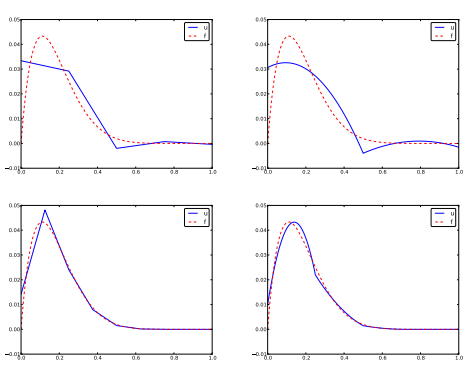
\includegraphics[width=0.7\linewidth]{img_29}
		\caption{Comparison of the finite element approximations: 4 P1 elements with
			5 nodes (upper left), 2 P2 elements with 5 nodes (upper right), 8 P1 elements
			with 9 nodes (lower left), and 4 P2 elements with 9 nodes (lower right).}
		\label{fig:img_29}
	\end{figure}
	\section[Sparse matrix storage and solution]{Sparse matrix storage and solution}
	\label{sec:sec_4_8}
	\noindent Some of the examples in the preceding section took several minutes to compute, even on small meshes consisting of up to eight elements. The main explanation for slow computations is unsuccessful symbolic integration: sympy may use a lot of energy on integrals like $\int f(x(X)) \tilde{\varphi}_{r}(X) h / 2 d x$ before giving up, and the program then resorts to numerical integration. Codes that can deal with a large number of basis functions and accept flexible choices of $f(x)$ should compute all integrals numerically and replace the matrix objects from sympy by the far more efficient array objects from numpy.
	
	Another reason for slow code is related to the fact that most of the matrix entries $A_{i, j}$ are zero, because $\left(\varphi_{i}, \varphi_{j}\right)=0$ unless $i$ and $j$ are nodes in the same element. A matrix whose majority of entries are zeros, is known as a sparse matrix. The sparsity should be utilized in software as it dramatically decreases the storage demands and the CPU-time needed to compute the solution of the linear system. This optimization is not critical in 1D problems where modern computers can afford computing with all the zeros in the complete square matrix, but in $2 \mathrm{D}$ and especially in 3D, sparse matrices are fundamental for feasible finite element computations.
	
	In 1D problems, using a numbering of nodes and elements from left to right
	over the domain, the assembled coefficient matrix has only a few diagonals
	different from zero. More precisely, 2d + 1 diagonals are different from zero.
	With a different numbering of global nodes, say a random ordering, the diagonal
	structure is lost, but the number of nonzero elements is unaltered. Figures \hyperref[fig:img_30]{30}
	and \hyperref[fig:img_31]{31} exemplify sparsity patterns.
	\begin{figure}[H]
		\centering
		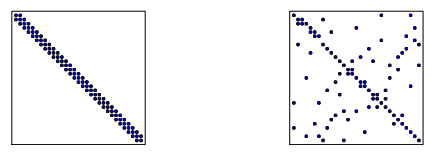
\includegraphics[width=0.7\linewidth]{img_30}
		\caption{Matrix sparsity pattern for left-to-right numbering (left) and random
			numbering (right) of nodes in P1 elements.}
		\label{fig:img_30}
	\end{figure}
	\begin{figure}[H]
		\centering
		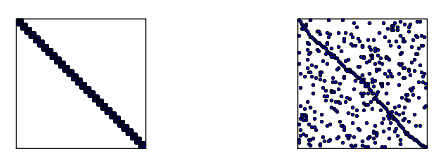
\includegraphics[width=0.7\linewidth]{img_31}
		\caption{Matrix sparsity pattern for left-to-right numbering (left) and random
			numbering (right) of nodes in P3 elements.}
		\label{fig:img_31}
	\end{figure}
	
	The scipy.sparse library supports creation of sparse matrices and linear system solution.
	\begin{itemize}
		\item scipy.sparse.diags for matrix defined via diagonals
		\item scipy.sparse.lil\textunderscore matrix for creation via setting matrix entries
		\item scipy.sparse.dok\textunderscore matrix for creation via setting matrix entries
	\end{itemize}
\clearpage
\end{document} 
